% Autonomous laboratory
% https://www.nature.com/articles/s41586-023-06734-w

% Accelerating material discovery
% https://www.nature.com/articles/s41524-022-00765-z

%High-throughput experiments facilitate materials innovation: A review
%https://link.springer.com/article/10.1007/s11431-018-9369-9#:~:text=High%2Dthroughput%20materials%20experiments%20including,at%20a%20fraction%20of%20cost.

\begin{figure*}[!ht]
    \centering
    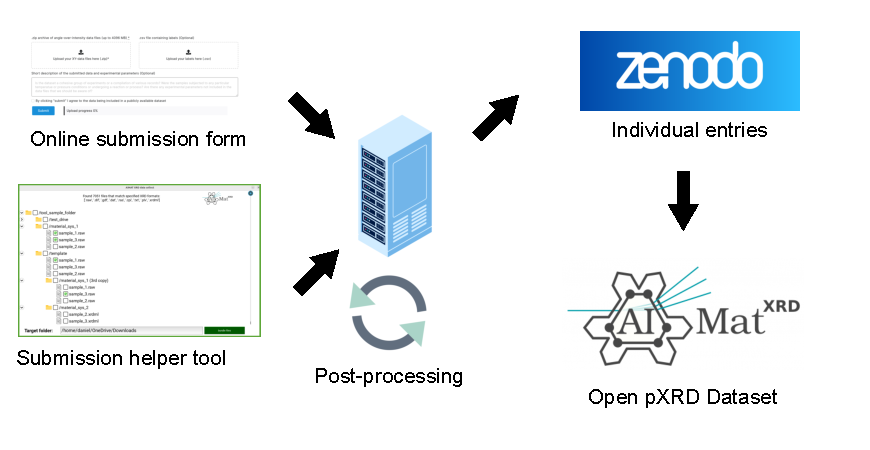
\includegraphics{figures/overview.pdf}
    \caption{Overview of the data collection pipeline. Datasets are submitted using an online submission form or our submission helper software. After post-processing and data homogenization, we create a Zenodo entry for each user submission and subsequently include the submission in the opXRD database.}
    \label{fig:overview}
\end{figure*}

The advent of high-throughput experiments holds the prospect of significantly accelerating the speed of materials discovery.
The synthesis and characterization of novel materials is becoming increasingly efficient and automated,
which increases the throughput of samples in experimentation pipelines.

% Rietveld Refinement (3.9 Profile fitting and rietveld analysis)
%https://www.sciencedirect.com/topics/biochemistry-genetics-and-molecular-biology/rietveld-refinement

% Rietveld Refinement: Half a century anniversary
% https://pubs.acs.org/doi/10.1021/acs.cgd.1c00854

% On Rietveld refinement
After fabricating a new material, a number of analysis techniques can be used to characterize the sample.
The most important method to determine the crystal structure of a new material is powder X-ray diffraction. 
%In the case of multi-phase samples, this includes identifying the phases present in the sample and quantifying their fractions.
To analyze pXRD data, an initial guess is optimized using Rietveld refinement. In this process, an initial crystal structure, including unit cell parameters, provided by the operator of the analysis software, is fitted to the observed diffractogram in an iterative optimization process based on simulated forward prediction of expected pXRD diffractograms given the current crystal structure.
%The unit cell parameters of the crystal structure are adjusted to minimize the difference between the simulated diffraction pattern and the pattern observed in the experiment. 
As Rietveld refinement is a local optimization method, the result of the refinement procedure is generally only as good as the initial guess it was provided with.
Therefore, it strongly relies on the experience of the operator to provide an accurate initial guess of the crystal structure.

Employing manually operated Rietveld refinement, including determining a good initial structure for the optimization, is not without issues.
It is certainly not scalable to the degree required to keep up with advances in throughput and efficiency in other steps of the experimentation pipeline.
Furthermore, initial guesses for Rietveld refinement are often obtained by matching the observed diffractogram to patterns from a database.
%But beyond the lack of scalability of this workflow we also wish to highlight the following issue:
%Providing the analysis software with an initial guess of the structure requires manually or algorithmically
%consulting a reference library of crystal structures with corresponding simulated or sometimes real diffractograms.
%From that reference library, a crystal structure must be identified that is likely to be similar
%to that of the investigated sample which can then serve as the initial guess provided to the analysis software.
%Since the number of chemically viable crystal structures is infinite, any such library will always be incomplete.
However, in the case of novel observed structure types, simply matching to a database of known structures will not yield good results. Therefore, more complex crystal structure solution approaches need to be applied to find suitable crystal structure guesses.
%The best that can be done to remedy this is to continually update the library both on the side
%of the distributor and the user, which is an undesirable overhead.
%Especially for novel material discovery, it may be impossible to find a sufficiently accurate match in the reference
%library to apply Rietveld Refinement successfully.

Machine learning has the potential to speed up the manual analysis of powder diffractograms and keep pace with an automated high-throughput experimentation environment.
%eliminate both the need for manual inputs and the need for reference
%libraries in powder x-ray diffraction analysis, resulting in a streamlined and automated analysis process that can
%keep pace with an automated high-throughput experimentation environment.
Models can be trained to predict crystal structure information directly given a diffractogram, or models can be used to automate the conventional workflow of finding an initial guess and running ML-automated Rietveld refinement.
%However, the current limiting factor is the availability of sufficiently large labeled datasets.
So far, however, due to an absence of labeled datasets with experimental diffractograms, machine learning in this domain has largely relied on diffractograms simulated from known structures (such as from the ICSD) or, most recently, from generated synthetic crystals.

Models trained on datasets with simulated diffractograms have already shown very strong performance in predicting
lattice parameters, spacegroup, and crystallite size from simulated diffractograms.
However, the performance substantially drops off when these models are applied to data originating from experiments [cite 2-3 papers, incl. ours].
The patterns observed in experiments suffer from a host of imperfections that need to be modeled accurately in order to be able to transfer models trained on simulated data to experimental patterns. This includes noise, background, preferred orientation of the sample, ...
Most approaches currently model these imperfections as a simple signal based on a heuristic functional form added to the simulated diffractograms.

At the moment, the number of openly available datasets for experimental powder data is very limited.
The main sources for experimental patterns are XXX, YYY, and ZZZ.
In this publication, we provide a new dataset that collects a broad range of patterns from experiment, exceeding the currently available amount of openly accessible experimental patterns by XX.
The dataset has been curated by collecting the accumulated powder data from multiple large research groups and institutions with high-throughput XRD facilities.

% How to contribute? This aspect deserves a separate paragraph
We further provide an online platform that can be used to easily submit new pXRD data to the dataset, which will be used to extend the existing dataset in the future (Figure~\ref{fig:overview}).
TODO: Make this longer?

Collecting a labeled dataset of raw experimental powder X-ray diffraction data of sufficient size to directly train a model that predicts crystal structure information is still out of reach.
The most advanced ML models currently are trained on approximately x simulated diffractograms, which is x orders of magnitude higher than the initial state of the opXRD database presented here.
However, our dataset still holds significant value in practice. First of all, the dataset can be used to better test and benchmark existing and new automated analysis approaches, which yields a better comparison than when using the very limited currently available datasets, such as the commonly used RRUFF mineral dataset.

Furthermore, we hope that our dataset can enable machine learning researchers to evaluate how closely their simulations
represent actual experimental data, identify what features are missing, and modify their simulation algorithms accordingly to arrive at a simulation that mirrors how data appears in reality.
One can bring the simulated patterns closer to experiment by improving the simulation itself by properly modeling more of the observed physical effects such as preferred orientation, peak shapes resulting from different sources, etc.
Additionally, some of the observed imperfections, such as background and noise, can be modeled using machine learning approaches.
This is similar to the concept of style transfer\cite{Gatys2016,Ganin2015} found in the domain of machine learning applied to images.
Here, the objective is to obtain a classification or regression model when only labeled images of one style (simulated data) and unlabeled or partially labeled images of another style (experimental data) are available.
The broad range of available experimental samples contained in our dataset makes it possible to apply these state-of-the-art ML approaches to the domain of powder XRD analysis.
We hope that this will yield more advanced automated ML approaches in the future, which can readily be applied in high-throughput experimentation pipelines.













%We hope that this will yield more attempts of ML-guided XRD analysis in the future, where also open challenges such as different angle step sizes, different radiation sources, will be addressed.

%However, there is still reason to believe that the strong performance observed in the domain of purely simulated diffractograms can to a large extent translate to predicting crystal structure properties from diffractograms originating from experiment, given that models are trained on a dataset that accurately reflects diffractograms as they appear in experiment.

%There are roughly speaking two paths towards improving the simulation: The first is to more accurately model the sample and the processes taking place within it during the simulation of the powder diffraction pattern. This would for example necessitate modelling absorption of the incoming X-ray radiation and its re-emission in the form of characteristic radiation and modeling the effect of stress and motion within the crystal on the diffractogram.

%An alternative route to obtaining a more accurate simulation is to try to learn these "imperfections" compared to an idealized simulation using machine learning techniques by extracting them from this dataset.

%As an example of this could be done, we can investigate results from other areas of research, where a transfer of data content between different "styles" of representation was attempted:

%Ganin et al.\cite{Ganin2015} proposed a mechanism for training a classifier which performs well independently of which style the input data is represented in, which only requires labeled data from one style and unlabeled data from other styles. This corresponds precisely to the situation at hand, where the number of labeled simulated diffractograms is virtually unlimited and a large amount of unlabeled real diffractograms are available, but labeled real diffractogram are in short suppply. This algorithm could be applied to train a "style-invariant" structure properties prediction model using a combination of our dataset and simulated labeled patterns.

%Another approach by Gatys et al. \cite{Gatys2016} achieves style transfer of images, by requiring that the content of the output image remain the same, while the style must match that of another image, chosen to represent the target style. This procedure could be applied to transfer the style of simulated diffractorams to that of real diffractograms, which could then be used to train the model data that is more faithful to powder diffractograms as they appear in experiment.

%A first hint of how closely a given simulation reflects experiment could be obtained by
%training a machine learning model, which attempts to classify between simulated and real diffractograms. \\
%If the simulation is very accurate, we would expect the classifier to not have few to no features which it can use to distinguish between simulated and real diffractograms and hence perform poorly. \\
%Conversely, if the classifier performs well and is not difficult to train, that would be an indicator that the simulation doesn't reflect experiment sufficiently well. \\

%For a set of given sample properties there is only one corresponding simulated diffractogram, but there may be an infinite amount of variations in how the diffractogram of a sample could look like in experiment for example due varying measurement apperatus, noise
%, sample impurities and lattice defects.
%In order for a simulated dataset to closely resemble experiment it is critical that the simulation also represents these
%statistical variations.
%Determining the nature of these variations is a much a harder task than making individual diffractograms look like they
%originated from experiment and cannot be accomplished by simply training a classifier.
%Nevertheless, we hope that this dataset can at least provide clues of how to take this aspect into account during
%simulation as well.

%But even the unlabeled portion of the dataset can be used to test the performance of models, if the model attempts to predict the entire crystal structure. From the predicted crystal structure, the corresponding diffractogram can be simulated, which can then be compared to the real diffractogram that was used as input for the prediction. While a nearly matching diffractogram doesn't necessarily mean a correctly predicted structure, a non-matching diffractogram certainly means an incorrectly predicted structure.

%Finally, by inviting the application of models to data as it appears in experiment we would like to bring attention
%to some of the practical difficulties that need to be addressed in applying a model to a wide variety of X-ray diffractograms
%collected from different sources: For example the angle and the step size of the diffractograms will differ between sources, 
%which is something that any model that aims to perform well on this dataset must be equipped to handle.

% TODOS:
% - This paper talks about the importance of sharing raw powder x-ray diffraction data. I'd definitely cite it ->  \cite{Aranda2018}
% - The image diff.png shows the difference between a powder diffractogram calculated from single x-ray diffraction data
% and a real powder diffractogram of the same material. The difference is enormous. I'd include it to highlight
% that simulating powder diffractino patterns from single crystal data only goes so far
%https://www.sciencedirect.com/topics/biochemistry-genetics-and-molecular-biology/rietveld-refinement

%-----------------------------------------------------------%
% Sources on rietveld refinement

% Computationally intensive -> Probably outdated. If it used to take minutes in 2010
% it probably only takes seconds by now.
% https://www.rigaku.com/de/node/707

% A simple solution to the Rietveld refinement recipe problem
% -> Rietveld refinement requires "expert input"
% https://www.ncbi.nlm.nih.gov/pmc/articles/PMC10840306/

% Comments -> Why having to do rietveld refinement sucks
% FullProf tutorial on fitting XRD peaks -> Tedious, requires lots of manual input
% https://pranabdas.github.io/research/fullprof/

% Topas tutorial -> 44 page tutorial, many boring and potentially frustrating steps, lots of points offer potential for task failure
% https://topas.webspace.durham.ac.uk/topas_user_menu/

%  Methods and Tutorials – Powder Diffraction -> Overview of rietveld refinement data
%https://neutrons.ornl.gov/sites/default/files/Methods%20and%20Tutorials%20Powder%20Diffraction.pdf

% Rietveld Refinement from Powder Diffraction Data -> 50 pg tutorial that no one wants to read, overwhelming amout of quantities/figures that needs to be manually looked at in the process
% https://www.fkf.mpg.de/4112052/cpd26.pdf